\chapter{Parallel Programming with OpenMP}
\label{chap:OpenMP}

Nowadays, every single CPU is multi-cores architecture. How to take advantage of
this, while current programming language is designed for sequential execution?
One important solution is using OpenMP.

\section{OpenMP}

OpenMP standard was formulated in 1997 as a method for writing portable,
multi-threaded applications. It started first as a Fortran-based standard, and
then was accepted in C/C++. Both task parallelism and data parallelism can be
achieved using OpenMP directives. The number of threads can be defined
(Sect.\ref{sec:set_num_threads}).

OpenMP 1.0 only for Fortran (1997), and OpenMP for C/C++ in 1998. In 2000,
OpenMP 2.0 was released for Fortran, and in 2002 for C/C++. OpenMP 2.5 for C/C++
and Fortran was released in 2005. OpenMP 3.0 was released in 2008. OpenMP 3.1
was released in 2011. OpenMP 4.0 is expected to be released in Jul, 2013.

\begin{mdframed}
OpenMP 2.0: supported by Microsoft Visual C++ 2005, Xbox 360 platform.
\begin{itemize}
  \item VC++ 2005 (DONOT support static linking): Configuration properties
  $\rightarrow$ C/C++ $\rightarrow$ Language, then modify OpenMP support property to invoke /openmp
  switch, which cause the compiler to define the symbol \verb!_OPENMP!. This
  macro is important in the code where we use \verb!#ifndef _OPENMP! to check
  for OPENMP support. OpenMP is linked to the application through import lib
  \verb!vcomp.lib!, with runtime library \verb!vcomp.dll!. The correspondingly
  debug version is \verb!vcompd.lib! and \verb!vcompd.dll!.
  \item Xbox 360 (support static linking): 
\end{itemize}
\end{mdframed}

OpenMP begins with a master thread, Fig.\ref{fig:OpenMP_concept}. As the program
executes, it may encounter parallel regions, at which the master thread creates
thread teams (which include the master thread). From within a parallel region,
there can be nested parallel regions where each thread of the original parallel
region becomes the master of its own thread team. Again, nested parallelism can
continue to further nest other parallel regions.
At the end of a parallel region, the thread teams are parked and the master
thread continues execution

 \begin{figure}[hbt]
  \centerline{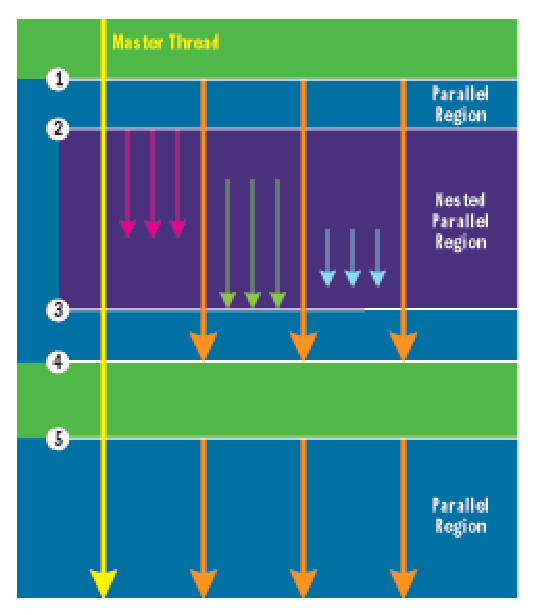
\includegraphics[height=5cm,
  angle=0]{./images/OpenMP_concept.eps}}
  \caption{OpenMP parallel sections}
  \label{fig:OpenMP_concept}
\end{figure}


\begin{figure}[hbt]
  \centerline{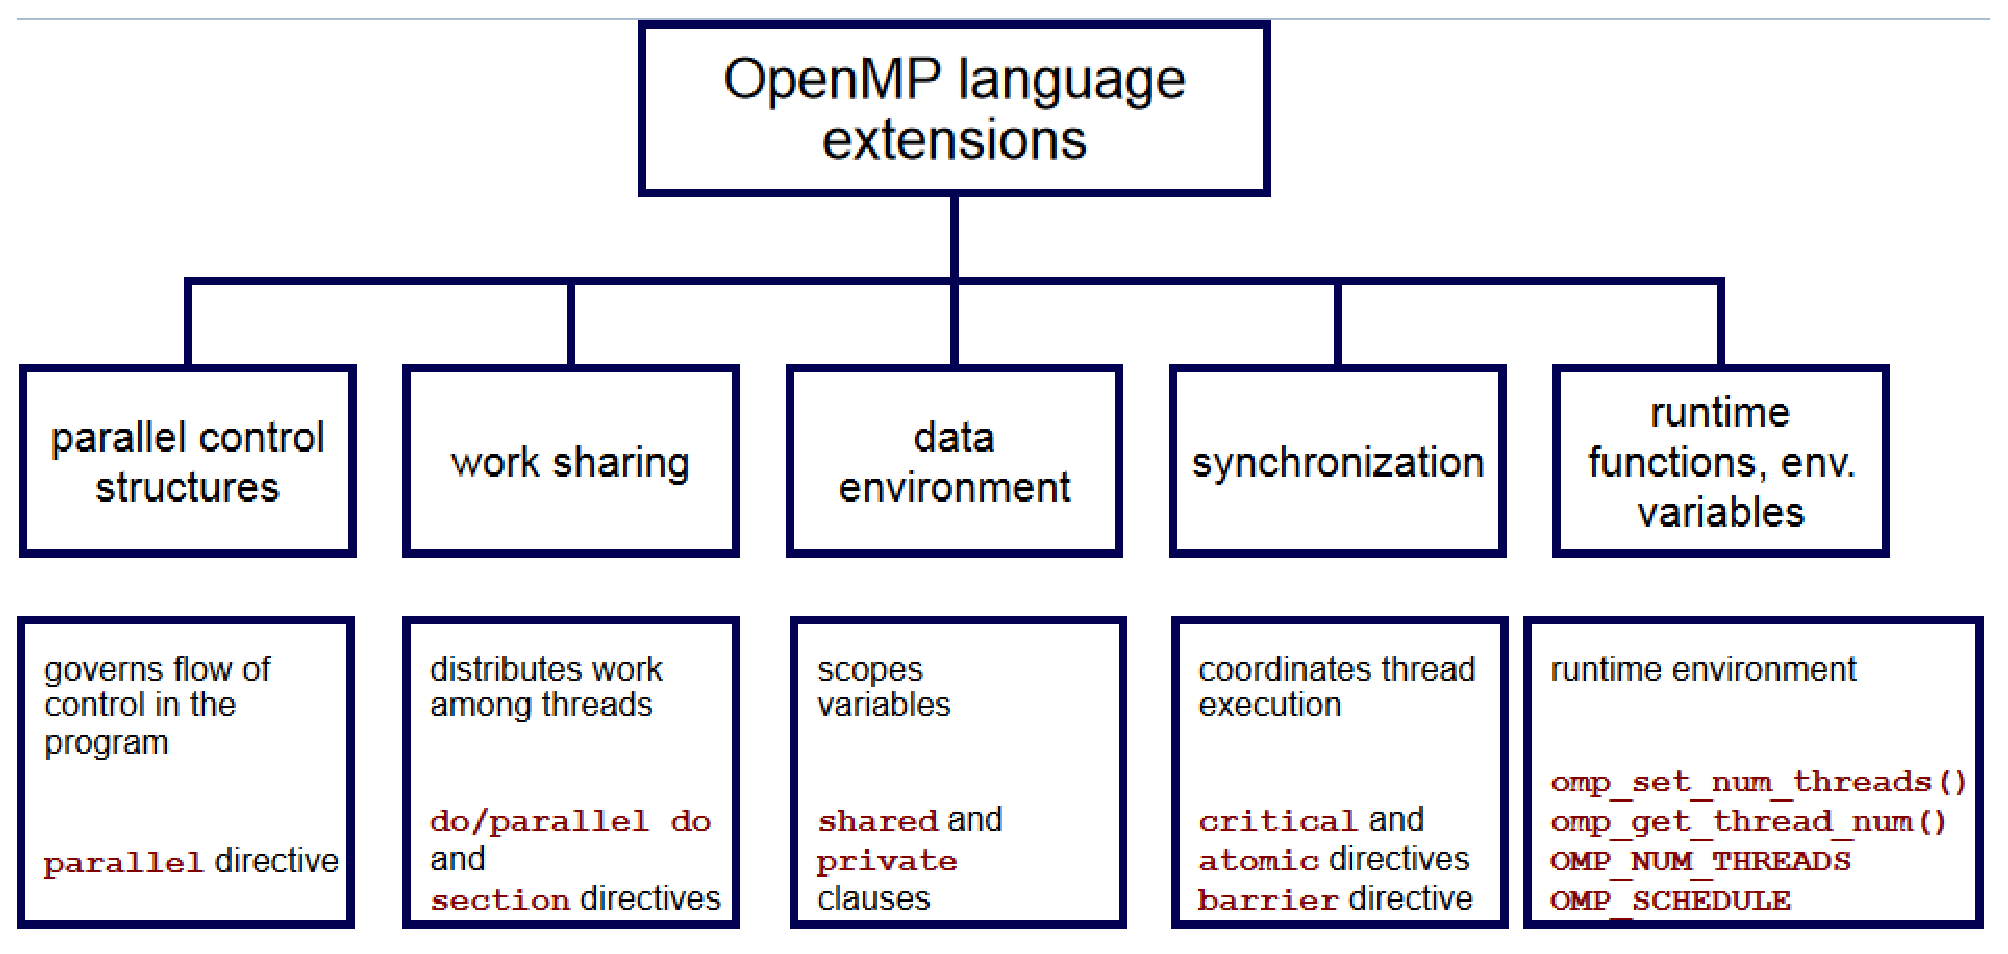
\includegraphics[height=5cm,
    angle=0]{./images/openMP_structure.eps}}
  \caption{OpenMP constructs}
\label{fig:OpenMP_core_elements}
\end{figure}

The core elements are the constructrs for thread creation, workload distribution
(work sharing), data-environment management, synchronization, and user-level
runtime functions, , Fig.\ref{fig:OpenMP_core_elements}. OpenMP consists of 2
basic constructs: pragmas and runtime routines. All OpenMP pragmas begin with
\verb!#pragma omp!.
\begin{verbatim}
#pragma omp <directive> [clause[ [,] clause]...]
\end{verbatim}

To use OpenMP, we need to include <omp.h> file
\begin{verbatim}
#include <omp.h>
\end{verbatim}
and depending the compiler, compile the code with 
\begin{itemize}
  \item \verb!-fopenmp!: GNU (gcc, g++, gfortran) with default behavior as many
  threads as available cores
  \item \verb!-openmp!: Intel (icc, ifort) with default behavior as many threads
  as available cores
  \item \verb!-mp! : Portland Group (pgf90, pgcc, pgCC, pgf77) with default
  behavior is 1 thread
\end{itemize}
To explicitly control the number of threads, see Sect.\ref{sec:set_num_threads}.

\subsection{OpenMP 2.5}

Support GNU Compiler 4.2+, MSV C++ 2005 (to enable add \verb!/openmp! to
commandline), Intel C 10.1 (use \verb!-openmp!, if enable but don't do actual
parallel execution use \verb!-openmp-stubs!).

\subsection{OpenMP 3.0}

Support GNU Compiler 4.4+, Intel C 11.0.

New features: the concept of \verb!task! and \verb!task! construct.

\subsection{OpenMP 3.1}


\subsection{OpenMP 4.0}

New features: support accelerators (heterogeneous computing), atomics
operations, error handling, thread affinity, tasking extensions, and user
defined reduction, SIMP support and Fortran 2003 support.


\section{Set number of threads}
\label{sec:set_num_threads}

The number of threads are set by the system (compilers) or can be overloaded by
environment variable or using code function. By default, the number of set is
given by the system or the compiler. Next, we can overload this using we set the
environment variable \verb!OMP_NUM_THREADS!.
\begin{verbatim}
export OMP_NUM_THREADS=4
\end{verbatim}

or at the highest level, in the code
\begin{verbatim}
#include <omp.h>

#define NUM_THREADS 4
omp_set_num_threads(NUM_THREADS);
\end{verbatim}



\section{Directives}
\label{sec:openmp_directives}

They are: parallel, for, parallel for, section, sections, single, master, critical, flush,
ordered, and atomic.

The directives can be classified into 2 forms:
\begin{enumerate}
  \item work-sharing directives: it do not create parallelism, but rather
  distribute the work into threads in the thread-team in a logical way to speed
  up the execution, i.e. the chunk of work to different threads must be
  independent.   They are:
  \verb!for!, \verb!ordered!, \verb!section!, \verb!sections!, \verb!single!.
  \item thread creation: \verb!parallel!
\end{enumerate}


\subsection{parallel ***}

This is the most important and most common directive, which create a parallel
region for the dynamic extent of the structured-block that follows
\begin{verbatim}
#pragma omp parallel [clause[ [, ]clause] ...] 
structured-block
\end{verbatim}
It tells the compiler that the code in the structured-block should be executed
in parallel on multiple threads. Each thread will execute on the 
instruction-stream, however not necessarily the same set of instructions. The
number of threads $N$ is chosen at runtime (Sect.\ref{sec:set_num_threads}).

Example:
\begin{verbatim}
#pragma omp parallel
{ 
    printf("Hello World\n");
    printf("ABC");
}
\end{verbatim}
If we don't put the block \verb!{  }!, only the next statement are put into
threads. Example:
\begin{verbatim}
#pragma omp parallel 
    printf("Hello World\n");
printf("ABC");  //only master do
\end{verbatim}

Depending on your setting, a number of threads will print out to the terminal
the two strings. As they share the  standard output, {\it race conditions}
may occur, i.e. the string are overlapped as character by character are
concurrently printed out by more than one thread.

\begin{mdframed}
Internally, GCC implements parallelism by creating amagic function and moving
the associated code into that function, and variables declared within that
blocks (or those declared outside but we ask to be private to each thread)
become local variables to the magic function (and thus, local to each thread).

Variables shared by threads are handled transparently, e.g. by passing reference
or using register variables which are flushed at the end of the parallel block
(or whenever \verb!flush! is executed).
\end{mdframed}

To be more specify in how the work should be distributed to threads, there are
additional clauses to be used
\begin{enumerate}
  \item \verb!for! or \verb!do!: $\rightarrow$ data parallelism 
  \item \verb!sections!: put consecutive (but independent) blocks of codes to
  different threads 
  \item \verb!single!: force only one thread to execute the code, a barrier is
  implied to the end
  \item \verb!master! : like \verb!single!, but ask the master thread to
  execute, and no barrier implied at the end.
\end{enumerate}

Parallelism can also be made {\it conditional}, i.e. depending on the value of
some logical expression, using  an \verb!if! clause
\begin{verbatim}
extern int some_value;

#pragma omp parallel for if (some_value)
for (int c=0; c<n; c++} {
		//do something
}

// NOTE: zero means false
\end{verbatim}

If we ignore \verb!parallel! keyword, then whatever threads available in the
current team is used to run the code in parallel. In the begining, the thread
team has only one member, the master thread. So
\begin{lstlisting}
#pragma omp for 
for (int i=0; i<n; i++){
	//do something
}
\end{lstlisting}
may be executed by only one thread, i.e. the master thread.

You can create a new thread team using 
\begin{lstlisting}
#pragma omp parallel 
{
   #pragma omp for 
   for (int i=0; i<n; i++){
      //do something
  }
	
  #pragma omp for
  for (int i=0; i<n; i++) {
      //do other things
  }

  SomeMoreCode(); //all threads execute this, but not before 
        // all threads complete the previous loop
        // NOTE: We can avoid this, i.e. allow whatever thread
        //      complete the loop to execute this code
        //      : by using 'nowait' clause in the previous #pragma
}
// always synchronize here

\end{lstlisting}
IMPORTANT: \verb!nowait! can only be used with \verb!sections!, \verb!for! and
\verb!single!. We can not use with \verb!parallel!, nor \verb!ordered! clause.

We can also specify exactly how many threads we want to create using clause
\verb!nu_threads(4)!.

\begin{verbatim}
#pragma omp parallel num_threads(4)
{


}
\end{verbatim}


More example:
\begin{verbatim}
#pragma omp parallel num_threads(2)
{
  Work1();
  #pragma omp single
  {
  	Work2();
  } //implied barrier here
  
  Work3();
}
\end{verbatim}
So, Work1() is done twice, Work2() is done once (by which thread is due to
implementation-defined, e.g. in GCC, \verb!libgomp! decides), and Work3() is
done twice. We can force the master thread to execute Work2() using
\verb!master! clause (and other threads free to execute Work3() without waiting)
\begin{verbatim}
#pragma omp master
{

} // no implicit barrier here
\end{verbatim}



\subsection{parallel + for $\rightarrow$ parallel for}
\label{sec:directive_for}

This is not what we want, as every thread does the full loop
\begin{verbatim}
#pragma omp parallel // probably not what was intended
{
for(int i = 1; i < size; ++i)
        x[i] = (y[i-1] + y[i+1])/2;
}
\end{verbatim}

What we want is that each thread does partial of the loop
\begin{verbatim}
#pragma omp parallel    
{
#pragma omp for
for(int i = 1; i < size; ++i)
        x[i] = (y[i-1] + y[i+1])/2;
}
\end{verbatim}
At the end of the parallel region, there is an {\it implicit} barrier
synchronization  that block there until the last thread completes.

Since this is the most common parallelized work-sharing construct, OpenMP
provides a short-hand 
\begin{verbatim}
#pragma omp parallel for
for(int i = 1; i < size; ++i)
    x[i] = (y[i-1] + y[i+1])/2;
\end{verbatim}

\textcolor{red}{IMPORTANT: The important of using work-sharing directives is
that we need to have a loop, and there is no dependency between iterations of
the loop.}


\verb!parallel for! or \verb!for! can be combined with some clauses:
\verb!reduction! (Sect.\ref{sec:clause_reduction})


\subsection{sections}
\label{sec:directive_sections}

\section{Data share/private}

OpenMP is the shared memory programming model, so any variable declared before
the thread creation are shared and seen by all threads. Sometimes, you want to
make them private to each thread (to avoid race conditions), we can tell the
compiler to generate new memory for these variable to each thread using data
sharing attribute clauses

\begin{enumerate}
  \item \verb!shared!
  \item \verb!private!
  \item \verb!default!
  \item \verb!firstprivate! : private and initialize to original value
  \item \verb!lastprivate!: private and original value is updated after
  construct
  \item \verb!reduction!: a safe way of joining work from all threads after the
  construct
\end{enumerate}

 By default

\section{Clauses}

\subsection{reduction}
\label{sec:clause_reduction}

\begin{verbatim}
reduction(operation:var)
\end{verbatim}


This clause can be used with some directives: \verb!for!
(Sect.\ref{sec:directive_for}), \verb!sections!
(Sect.\ref{sec:directive_sections}).


\section{Synchronization}

With multiple threads running concurrently, it's sometimes that we need to
synchronize one thread with another. One common situations is at the end of the
parallel region, before the sequential code can be executed by the master
thread, an implicit barrier synchronization is given to wait for all threads in
the thread-team to complete. 

Other places with implied barrier synchronization, at the end of each 
\verb!#pragma omp for!, \verb!#pragma omp single!, and 
\verb!#pragma omp sections! block. To remove implied barrier synchronization, we
use \verb!nowait! clause
\begin{verbatim}
#pragma omp parallel    
{
    #pragma omp for nowait
    for(int i = 1; i < size; ++i)
        x[i] = (y[i-1] + y[i+1])/2;
} // implicit barrier here

CodeWork();
\end{verbatim}

To causes all threads to wait until all other threads in the same team reach a
certain point, we put a single line with
\begin{verbatim}
#pragma omp parallel
{
   SomeCode();
   
   #pragma omp barrier
   
   // All threads need to complete SomeCode()
   // before can execute here
   SomeMoreCode();  
\end{verbatim}
to tell all threads in the thread-team to reach here before parallel execution
can be continue.
